\chapter{国内外研究现状及解决方案}\label{chap:RelateWorkSolvMethod}

\section{国内外研究现状}

话题检测最早起源于面向事件的检测与跟踪(Event Detection and Tracking,EDT),距今已经20多年了。EDT主要检测一个特定时间发生的特定事件。然后由事件扩展演化出话题的概念,出现了话题检测与追踪任务(Topic Detection and Tracking,TDT)\citep{allan-1998-TDT}。与EDT不同,TDT从传统对于事件的检测追踪转移到对包含突发事件及其后续报道的话题的检测与追踪。

TDT定义话题是一个核心事件或活动以及与之直接相关的事件或活动。由于当时互联网并不普及,用户更多的是通过新闻报道来了解外部世界,导致当时研究重点是自动发现新闻报道流中的话题,再按话题组织各种事件及其相应的报道。所以,TDT的主要任务就是对新闻报道进行话题检测与追踪。新闻报道大都经过专业人士创作和编辑,具有主题明确、内容正规、用词准确、噪声小、易于处理等特点。

对于纯文本数据的话题检测,主要使用自然语言处理方法,比如提取新闻文本的TF-IDF特征(Term Frequency,Inversed Document Frequency)\citep{salton1988tfidf}来构建特征向量,然后通过简单的聚类算法,生成的每个聚类就是一个话题。但是由于单纯的词汇统计特征并没有考虑词之间的语义关系,所以这些方法往往结果很差。考虑到文本数据中词之间的语义关联以及话题的语义性,有研究者提出了主题模型(Topic Model)。主题即我们所要检测的话题。这类模型认为文档不应该完全归属某一类,而是根据一定概率分布在隐含主题上,同时认为每个隐含主题包含多个词。其中有三个经典的主题模型:LSA、PLSA和LDA。

隐语义分析(Latent Semantic Analysis,LSA)\citep{deerwester1990indexing}最初用在语义检索上,目的是为了找出词在文档和查询中真正的含义,也就是隐含语义,从而解决一词多义和一义多词的问题。LSA和传统的向量空间模型一样使用向量来表示词和文档,并通过向量之间的的关系来判断词之间以及文档之间的关系。不同的是,传统的向量空间模型使用精确的词匹配,即精确匹配用户输入的词与向量空间中存在的词,无法解决一词多义和一义多词的问题。因为在实际匹配中,我们想要比较的不是词,而是隐藏在词后面的意义和概念。而LSA将词和文档从高维空间映射到低维的语义空间,再比较其相似性。从而解决一词多义和一义多词的问题,并且去除了原始向量空间中的一些噪声,提高特征的鲁棒性。实际上,如图\ref{fig:lsa}所示,LSA使用奇异值分解(Singular Value Decomposition,SVD)技术将文档-词汇矩阵$A$分解为词汇-话题矩阵$U$、话题-话题矩阵$S$、文档-话题矩阵$V$,从而挖掘出隐含的主题语义。再通过选择奇异值中最大的$t$个数,且只保留矩阵$U$和矩阵$V$的前$t$列来降维,从而达到过滤噪声和冗余数据的目的。最后基于这三个矩阵可以做语义检索、词分类和文档分类(即话题检测)。
\begin{figure}[!htbp]
    \centering
    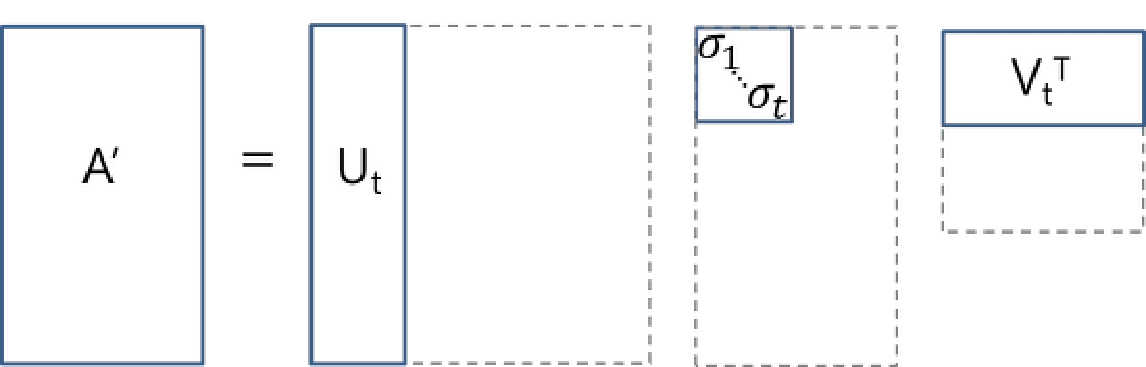
\includegraphics[width=0.70\textwidth]{lsa.pdf}
    \caption{LSA使用SVD分解原理图}
    \label{fig:lsa}
\end{figure}

概率隐语义分析(Probability Latent Semantic Analysis,PLSA)\citep{Hofmann1999PLSA}与LSA基础思想一致,都是希望找出词隐含的语义。二者区别在于LSA缺乏严谨的数理统计基础,且没有明确的物理解释,使用SVD分解操作。而PLSA使用概率模型,具有更明确的物理意义,并且使用期望最大化算法(Expectation-Maximization,EM)来学习模型参数。PLSA在文档和词之间构造隐含主题。PLSA认为一篇文档通常由多个隐含主题构成,而每个隐含主题由多个与该主题最相关的词来描述。即文档以一定的概率选择隐含主题,隐含主题以一定的概率选择词。PLSA建模思想简单,针对观察到的变量使用似然函数建模。建模中暴露出隐含变量,难以直接使用极大似然估计,所以使用EM算法求解。PLSA原理如图\ref{fig:plsa}所示。
\begin{figure}[!htbp]
    \centering
    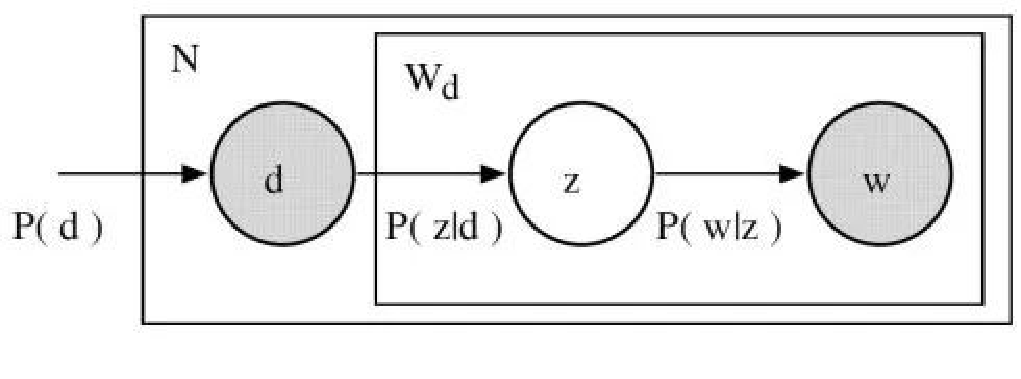
\includegraphics[width=0.70\textwidth]{plsa.pdf}
    \caption{PLSA原理图}
    \label{fig:plsa}
\end{figure}

隐狄利克雷分布(Latent Dirichlet Allocation,LDA)\citep{blei-2003-LDA}是PLSA的泛化版本。LDA认为文档到主题服从多项式分布,主题到词也服从多项式分布。LDA将PLSA中的参数变成随机变量,并且加入狄利克雷先验得到贝叶斯模型。使用狄利克雷先验主要是利用了狄利克雷分布和多项式分布的共轭性,方便计算。当将LDA的超参数设为特定值时,就特化成PLSA。LDA与PLSA的本质区别是估计参数的思想不同,PLSA使用频率派的思想,LDA使用贝叶斯派的思想。LDA的原理如图\ref{fig:lda}所示。其中$\alpha$和$\beta$是两个不同的狄利克雷分布的参数,分别用来生成隐含主题的分布参数$\theta$和词的分布参数$\varphi$。$z$和$w$分别是从各自分布中选出的隐含主题和特定的单词。
\begin{figure}[!htbp]
    \centering
    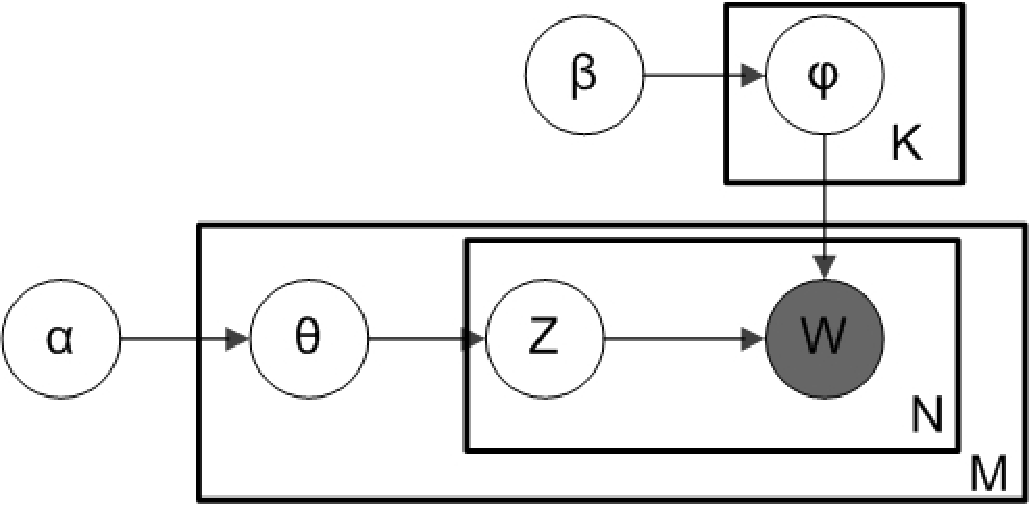
\includegraphics[width=0.70\textwidth]{lda.pdf}
    \caption{LDA原理图}
    \label{fig:lda}
\end{figure}

除了上述三种主题模型外,还有层级狄利克雷过程(Hierarchical Dirichlet Processes,HDP)\citep{the2006hierarchical}及各种主题模型的变种。这些主题模型通常在长文本上效果较好。然而,在短文本的网络数据中的效果却非常差。这是因为短文本导致词共现较少,而这些主题模型严重依赖于词的共现性,所以主题模型不能直接用来对稀疏的网络数据进行话题检测。

同时,网络数据不再是单一模态的文本数据,更多的是诸如文本、图片、音频、视频等多模态的异构数据的融合。针对多模态数据,许多文献将网络话题检测任务当做基于多模态数据的聚类任务。有两个主流的研究路线。一个是基于多模态的方法\citep{blei-lafferty-2007-correlatedtopicmodel,putthividhy-2010-multimodalLDA},另一个是基于相似度图的方法\cite{papadopoulos-2011-cluster}。

在基于多模态方法中,网络话题检测主要有两种研究方法:第一个研究方法是在多个模态的数据上进行聚类算法的研究。这种方法主要是将单模态的方法扩展到多模态数据。比如由LDA演变而来的多模态的LDA\citep{putthividhy-2010-multimodalLDA}提出从图片及其标签来检测话题。第二个研究方法是将多个模态的信息进行融合,再在融合后的信息上进行研究\cite{jia2011learning,Oh2014multimedia}。这种方法通过融合不同模态的信息以获得更大的信息量,再通过聚类算法检测网络话题。

在基于相似度图的方法中,多模态数据被融合进图中的边,然后将图中的顶点聚类成不同的话题。例如,Wu等人在论文\citep{wu-2007-crosslingual}中通过融合来自近似重复帧(Nearly-Duplicated Keyframes,NDKs)和演讲手稿的相似度来检测新闻视频中的话题。与基于多模态的主题模型相比,基于相似度图的方法可以很容易地扩展到其他算法\citep{cao-2011-tracking,aiello-2013-sensing,papadopoulos-2011-cluster}。

在聚类过程时,当前比较流行的聚类定义是计算话题内部的相似度。例如,Pang等人在\citep{pang-2013-unsupervised}使用相似度图中的最大团当作话题。Wang等人在\citep{wang2008automatic}中使用基于成对相似度的凝聚类算法来发现新闻中的话题。Cao等人在\citep{cao-2011-tracking}中通过k-means聚类算法在视频及其标签融合的相似度图上进行聚类。Zhang等人在\citep{zhang2013cross}中提出使用图转移(Graph Shift,GS)\citep{liu2010graphshift}算法来寻找密集子图作为话题。这些类内相似度方法通常只能发现一小部分热点话题,导致召回率相当低。因为简单的类内相似度方法并不能很好地解决当前稀疏并且充满噪声的网络数据。

与单纯计算类内相似度相反,一些方法采用了高级的聚类算法。论文\citep{xu2003document}使用非负矩阵分解算法(Nonnegative Matrix Factorization,NMF)来进行话题检测。与在文档上使用谱聚类算法相比,性能更好。然而这些高级方法在面对网络数据这种大规模的数据集时显得有些力不从心。无论是谱聚类算法还是非负矩阵分解算法,针对大规模数据时的复杂度非常高,导致网络话题检测效率很差。

实际上,由于网络数据的稀疏性以及高噪性,导致网络话题并不等同于聚类\citep{cao-2011-tracking}。因此,Pang等人在论文\cite{pang-2013-unsupervised}中将网络话题检测问题转化为无监督的排序问题,并提出PD算法来对话题权重进行计算。PD算法通过已有的聚类算法\citep{yang2012clustering,li2007noise}来获得过完备的话题集合,然后计算话题兴趣度,最后通过对话题的兴趣度进行排序来检测热点话题。然而,对PD算法来说,在大规模网络数据中产生过完备话题是一个非常耗时的过程\citep{pang-2013-unsupervised,pang-tao-2016-lpd}。

尽管许多方法提出解决大规模数据的话题检测问题,但是,据我们目前所知,只有一些方法试图通过并行LDA\citep{chen-2015-WarpLDA,wang-2009-PLDA,Liu-2011-PLDA+}来解决。正如在\citep{pang-2013-unsupervised,pang-tao-2016-lpd}所讨论的,LDA假设每个网页至少属于一个话题。然而,就网络数据而言,几乎有95\%的网页不能组织成话题。因此,并行化的LDA不能去除网络数据中所包含的大量的噪声网页。



\section{解决方案}

本论文研究面向大规模网络数据的话题检测。主要解决两方面问题,一个是针对网络话题的特点产生的问题,另一个是针对网络数据特点产生的问题。这些问题统计如下:
\begin{enumerate}
	\item[1] 针对网络话题特点而产生的问题:
		\begin{enumerate}
			\item[(1)] 话题大小不确定性问题:主要由于每个人对话题的认识不同,导致话题大小的界定有差异;
			\item[(2)] 话题数量不确定性问题:同样是由于每个人对话题的认识不同,导致话题之间的界限不明确;
		\end{enumerate}
	\item[2] 针对网络数据特点而产生的问题:
		\begin{enumerate}
			\item[(1)] 低质量的特征表示问题:主要是由于短文本的网络数据导致稀疏的特征表示;
			\item[(2)] 大量的噪声数据问题:主要是由于网络数据受到较少约束导致的大量错误、冗余、无关的数据。
			\item[(3)] 大规模的数据问题:主要是由于人能够便捷地网络上随意创作而带来的网络数据的爆炸式增长。
		\end{enumerate}
\end{enumerate}

基于上述问题,我们调研了目前国内外关于话题检测的相关文献。发现当前解决网络话题检测问题的比较优秀的方法是Pang等人在论文\citep{pang-2013-unsupervised}中提出的基于无监督排序的网络话题检测算法。该算法将网络话题检测问题转换为无监督的多粒度话题排序问题,从而避免了确定话题数量和大小的问题。该算法主要分为三个阶段:构造相似度图、生成多粒度话题、通过无监督排序确定真实话题。其中在构造相似度图时只保留最相近的$knn$个网页,从而达到过滤噪声的目的。然后在多级相似度图上使用最大团算法(Maximum Clique, MC)生成多粒度话题。最后在相似度图上基于泊松分布实现泊松去卷积算法来计算话题权重。虽然该论文最终比其他传统方法取得更好的结果,然而没有解决低质量的特征表示问题和大规模数据问题。

随后,Pang等人在\citep{pang-tao-2016-lpd}中通过融合多模态信息来提高特征质量,并且采用了更高级的聚类算法——基于随机游走的非负矩阵分解算法(Nonnegative Matrix Factorization Using Random Walk, NMFR)来生成多粒度话题。然而NMFR算法虽然能够提高聚类质量,但是同时也带来很高的时间复杂度。所以该论文还是没有解决大规模网络数据问题。

因此,本论文试图改进Pang等人提出的基于无监督排序的网络话题检测算法,以便更好地处理大规模网络数据。也就是说,本论文的最终目的是解决该算法的可扩展性问题。因此,我们主要针对该算法的两个部分进行改进。

\subsection{生成多粒度话题}

Pang等人使用过MC算法和NMFR算法在多级相似度图上生成多粒度话题。然而这两个算法都是非常耗时的算法,无法高效地处理大规模网络数据。跟传统方法一样,MC算法采用了一个看似合理的假设:相同话题内的网页之间的类内相似度应该大于话题内的网页和噪声网页之间的类间相似度。然而,由于低质量的特征表示以及语义鸿沟等问题导致这个假设站不住脚。与此同时,我们在研究真实话题在相似度空间的统计模式后,发现网络话题的组织模式与L\'evy Walks存在统计意义上的相似性\citep{perkins2014ascaling}。具体的,如果我们将网页间的相似度类比为L\'evy Walks中的步长,那么一个话题内的相似度分布符合重尾分布,而重尾分布被用来定性L\'evy Walks中的步长。

L\'evy Walks\citep{viswanathan2001levy,rhee2011levywalk}是随机游走模型中的一种。其中的步长服从某种重尾的概率分布。L\'evy Walks中的$flight$定义为一个质点从一个位置无偏移地移动另一个位置的步长。如图\ref{fig:levywalks}展示了L\'evy Walks中的$fligh$分别从柯西分布和正太分布中采样1000次的结果。直观上讲,L\'evy Walks包含许多较短的$flight$和一些额外较长的$flight$。因此,L\'evy Walks可以被用来描述诸如蜘蛛猴这样觅食动物的迁徙模式\citep{viswanathan2001levy}。同时,L\'evy Walks提供了一种更为有效的访问结点的方法\citep{li2010towards}。L\'evy Walks的另一个重要应用是在一个网络中路由\citep{perkins2014ascaling}。
\begin{figure}[!htbp]
    \centering
    \begin{subfigure}[b]{0.5\textwidth}
      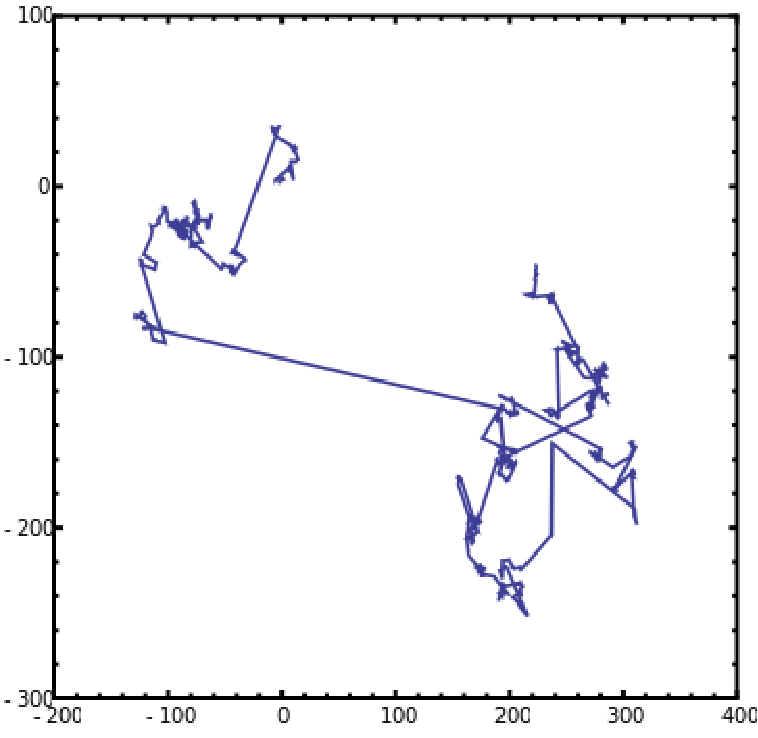
\includegraphics[width=\textwidth,height=0.9\textwidth]{CauchyDistribution}
      \caption{步长服从柯西分布}
      \label{fig:CauchyDistribution}
    \end{subfigure}%
    \begin{subfigure}[b]{0.5\textwidth}
      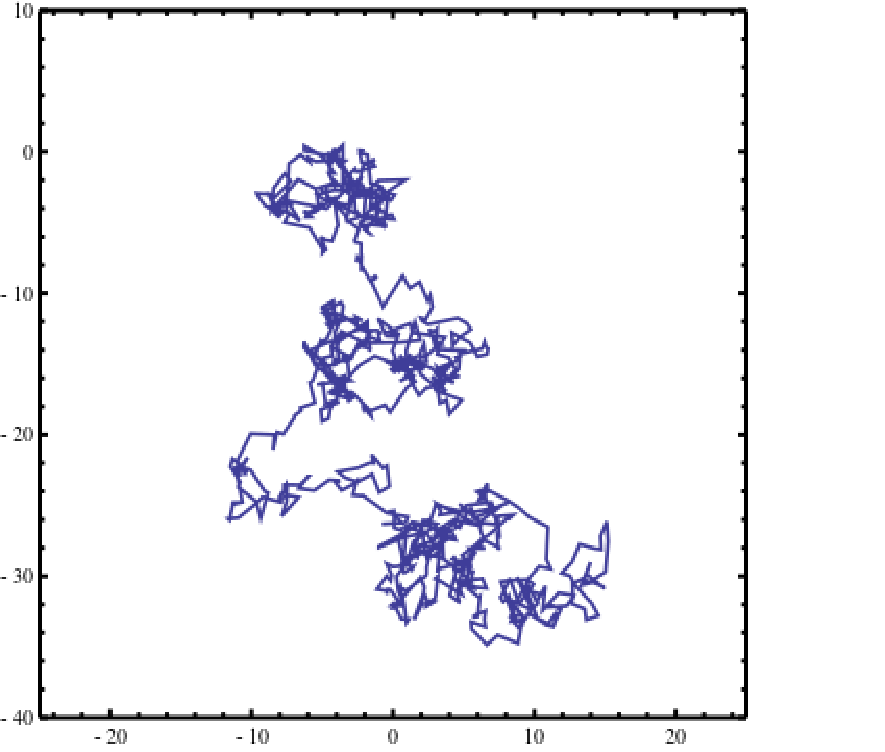
\includegraphics[width=\textwidth,height=0.9\textwidth]{BrownianMotion}
      \caption{步长服从正太分布}
      \label{fig:BrownianMotion}
    \end{subfigure}
    \caption{1000步L\'evy flight在二维坐标上的例子}
    \label{fig:levywalks}
\end{figure}

当L\'evy Walks被用来组织网络话题时,关键问题变成:1)如何在未知分布参数情况下模拟L\'evy Walks中额外较长的步长;2)如何确定所需步长的数量来组织话题;3)如何快速处理大规模的网络数据。基于上述3个问题,我们提出提出了下面对应解决方案:
\begin{enumerate}
	\item[(1)] 我们采用了一种基于种子话题的网页多分配算法来模拟相似度空间中的L\'evy Walks,优雅地避免了确定未知参数的麻烦;
	\item[(2)] 我们采用了层级阈值的方法来截断话题的生长,从而产生一系列过完备的话题,保证了话题的召回率;
	\item[(3)] 我们提出的网页多分配算法只需要进行简单的计算和分配,是一种无模型并且无需复杂参数优化的网络话题快速生成算法,从而向大规模网络数据的处理迈进了一步。
\end{enumerate}

据我们所知,本论文是第一个发现L\'evy Walks和网络话题在相似度空间上具有相似性。并且呈现了一系列完整的实验来证明这个发现对于网络话题检测的好处。我们提出的方法在计算上很简单但是效果非常好。仅仅通过简单的选择种子网页并且将网页分配到由种子网页生成的多个最相似的话题,无需进一步的参数调整等操作,我们找到一个新的组织网络话题的方式。并且在话题生成质量上比得上当前最好的方法,同时在话题生成效率上大大超过当前最好的方法。



\subsection{无监督排序}

Pang等人在论文\citep{pang-2013-unsupervised}中基于泊松分布假设提出泊松去卷积算法(Poisson Deconvolution,PD)。PD算法通过扩散网页之间的相似度来对每个话题分配一个权重。虽然相似度图可以通过在线$k$近邻图($k$-Nearest Neighborhood Graph, $k$N$^2$G)\citep{debatty-2016-fastonlineknn}构建,同时也可以通过稀疏矩阵的方式来高效的存储。但是,一个严重的问题是PD算法无法高效地处理大规模的网络数据。因为PD算法在每一轮必须使用所有数据在内存中重构一个$N\times N$的浮点型矩阵,其中$N$是网页数量。

那么我们是否可以在每一轮迭代更新时只使用一小部分数据来更新呢?一个简单但是有效的方法是随机优化\citep{hannah-2015-Stochastic}。这类方法至少能带来两个好处:1)减少物理内存的要求;2)避免一个$N\times N$规模的相似度图的重构。例如随机梯度下降(Stochastic Gradient Descent,SGD)及其变种\citep{Roux-2012-sgd-exponential,johnson-2013-sgd-accelerating,Nitanda-2014-sgd-proximal}由于优秀的效果和效率,已经广泛应用于机器学习。然而,通过EM算法优化的PD算法需要保持一个和相似度图同等规模的隐变量,并且PD算法的目标函数在每轮迭代时随着期望变化而变化。所以SGD算法并不能够解决基于EM算法优化的PD算法。

优化最小化原则(Majorization Minimization,MM)\citep{lange-2000-optimization}是EM算法的泛化版本。取目标函数的上界作为代理函数,然后迭代地最小化代理函数。许多方法可以用MM原则来解释,例如变分贝叶斯(Variational Bayes)
\citep{Wainwright-2008-variational-bayes}和近端算法(Proximal Algorithm)\citep{beck-2009-fastshrinkage}。随后,论文\citep{mairal-2013-SMM}提出随机优化最小化原则(Stochastic Majorization Minimization,SMM)使得MM具有可扩展性。

受到SMM的启发,我们提出随机泊松去卷积算法(Stochastic Poisson Deconvolution,SPD)来对PD算法进行可扩展性改造。SPD迭代地更新目标函数上界构成的代理函数。最终的SPD算法不仅只需要存储一小部分采样边,而且极大地加速了算法的收敛速度。

据我们所知,本文是第一个致力于解决PD算法的可扩展性问题,并将基于代理函数的优化原则用于PD算法中。提出的SPD算法不仅概念上简单,而且非常有效。